\section{Introduction}
\label{sec:intro}

Heliophysics as a discipline is the study of the Sun and its interactions with the solar system.
The Heliophysics community includes many people studying various sub-domains: the Sun, the solar wind, space weather, terrestrial and planetary magnetospheres, the heliosphere, and the Earth's ionosphere, thermosphere, and mesosphere.
Advancing our understanding of the fundamental processes underpinning this complex system requires interdisciplinary research across these scientific sub-disciplines.
At the time of writing, the NASA Heliophysics System Observatory consists of 18 missions with nearly 200 instruments.

Software packages to analyze data from these instruments are generally developed independently by each instrument team.
This creates a diverse and therefore difficult data and software environment to navigate.
Scientists conducting interdisciplinary research from multiple instruments run into problems with incompatible data formats and incompatible analysis routines written with different versions of the base code. Further, it is difficult to reproduce others' scientific results without open data and version-controlled open source software.

A common, version-controlled, open source platform that provides a standard interface to data products and encourages the re-use of common functions can go a long way toward solving this problem.
\sunpy aims to provide this solution for the field of solar physics.

The mission statement of the \sunpyproj is to facilitate and promote the use and development of several community-led, free, and open-source\footnote{\url{https://opensource.org/osd}} data analysis software packages based on the scientific \python\footnote{\url{https://www.python.org/}} environment.
To achieve this goal, the project primarily develops and maintains a core package (\sunpypkg) and supports an ecosystem of affiliated packages (see Section \ref{sec:affil_packages}) that provides additional functionality.

The \sunpyproj was formally founded in March of 2014.
The project selected the \python programming language to leverage the rich ecosystem of packages already available for general data analysis.
These include \package{Numpy} for multi-dimensional array manipulation \citep{numpy}, \package{scipy} for scientific functions \citep{scipy}, \package{Matplotlib} for publication-quality 2D plotting \citep{matplotlib}, and \package{Pandas} for data structures and time series analysis \citep{pandas}.
These core packages form the backbone for hundreds of thousands of additional \python packages.
Of particular relevance to \sunpypkg is the \astropypkg package, which provides core functionality for the analysis of astrophysical data \citep{astropy2018}.

This paper describes the first stable release (v1.0) of the core package.
A previous paper described release v0.5 \citep{Community:2015cy}.

\section{Project Organization \& Enhancement Proposals}

The organization of the \sunpyproj is modeled on the structure of a board-only not-for-profit corporate entity.
It consists of an up-to 10 member self-selected board.
An executive director, elected by the board, forms the core development team, leads the development of \sunpy core package, provides user support, and supports the development of affiliated packages.
As such, the executive director is also the \sunpy lead developer.
A deputy lead developer and release manager, as well as other volunteers from the developer community, support the lead developer.
Board members serve two year terms while the lead developer serves one year terms.

The \sunpyproj is formally defined through \sunpy Enhancement Proposals (SEPs) which are modeled after the Python Enhancement Proposal process\footnote{\url{https://www.python.org/dev/peps/}}.
SEPs are version controlled and publicly available\footnote{\url{https://github.com/sunpy/sunpy-SEP}}.
The first two SEPs (SEP-0001 and SEP-0002) define themselves as well as the \sunpy organization.

SEPs are used to both define the Project as a whole as well as technical requirements for the \sunpypkg core package.
There are generally three types of SEPs.
\begin{itemize}
    \item \textbf{Standard}: Introduces and describes a new feature, or changes to an existing feature, and is meant to function as a high-level technical design document.
    \item \textbf{Process}: Describes a new process, or changes to an existing process, in the \sunpyproj management.
    \item \textbf{Informational}: Provides information and does not introduce any new features, changes, or processes.
\end{itemize}

As of the time of writing, there are a total of 8 SEPs.
Some notable SEPs led to the adoption of physical units throughout the code base (SEP-0003, see Section~\ref{sec:units}), defined the affiliated package program (SEP-0004, see Section~\ref{sec:affil_package}), standardized the use of coordinate and coordinate transformations (SEP-0005, see Section~\ref{sec:coords}), and led to the adoption of a high precision scientific time format (SEP-0008).

\section{Support \& Sustainability}

The \sunpyproj relies largely on unpaid, volunteer efforts from early career scientists.
The project has not received any significant direct financial support for its work facilitating and promoting any open-source and open development software including \sunpy itself.
The \astropy community faces a similar problem \citep{PriceWhelan:2018ji, Muna2016}.

The \sunpyproj does participate in two summer of code programs, which offer students stipends to write code for open-source projects, via the OpenAstronomy umbrella organization.
Since 2013, 16 students contributed to \sunpy through the Google Summer of Code (GSoC)\footnote{\url{https://summerofcode.withgoogle.com/}} program.
Since 2011, 7 students contributed to \sunpy through a similar program funded by the European Space Agency called The ESA Summer of Code in Space\footnote{\url{https://socis.esa.int/}}.
Many \sunpy community members served as mentors for these students\footnote{\url{https://github.com/sunpy/sunpy/wiki/Wall-of-Fame}}.
In 2018, NumFOCUS, a 501(c)(3) public charity which collects and manages tax-deductible contributions for many open-source scientific software packages such as NumPy and AstroPy, gave GSoC student Vishnunarayan K. I. an award for exceptional contributions to the open source scientific software ecosystem for his efforts to update \sunpy with a modern astronomical time system.

The National Academies of Sciences, Engineering, and Medicine's report on Open Source Software Policy Options for NASA Earth and Space Sciences \citep{NAP2018} outlines several solutions to alleviate this problem -- namely that the NASA Science Mission Directorate provide funding for new and existing open source software projects, promote scientists who spend time developing and improving open source software projects, and offer prizes for exemplary contributions to the open source software community.
The National Academies of Sciences, Engineering, and Medicine's report on Reproducibility and Replicability in Science \citep{NAP2019} recommends that funding agencies invest in the research and development of open-source software that support reproducibility.
The \sunpy community supports solutions like these for all relevant funding agencies and furthermore has the ability to accept financial contributions from institutions or individuals through the NumFOCUS organization.

\section{Development Model}

To satisfy the mission statement of the Project, the \sunpy community adopted an open development model.
This development model is widely used within the scientific Python community.
The \sunpy organization and \sunpypkg package are hosted on \github and use Git\footnote{\url{https://git-scm.com/}} as its distributed version control software.
The entire codebase is publicly available and anyone can suggest changes through pull requests.
Since the codebase is licensed under a permissive 2-clause BSD licence\footnote{\url{https://opensource.org/licenses/BSD-2-Clause}}, anyone can redistribute, improve, repackage or use it in a closed environment as long as they credit the \sunpy developers and redistribute the license.
In order to maintain high quality code, every contribution must satisfy the following requirements:
\begin{enumerate}
    \item Code and documentation must follow widely used style guides (PEP 8 and numpydoc).
    \item All new features must be accompanied with documentation.
    This includes code comments, formal documentation, and gallery examples.
    \item Test code must be provided with coverage reports.
    \item Finally, all code must be reviewed and accepted by at least two members of the developer community before it is integrated into the codebase.
\end{enumerate}

\begin{figure}
\begin{tabular}{cc}
  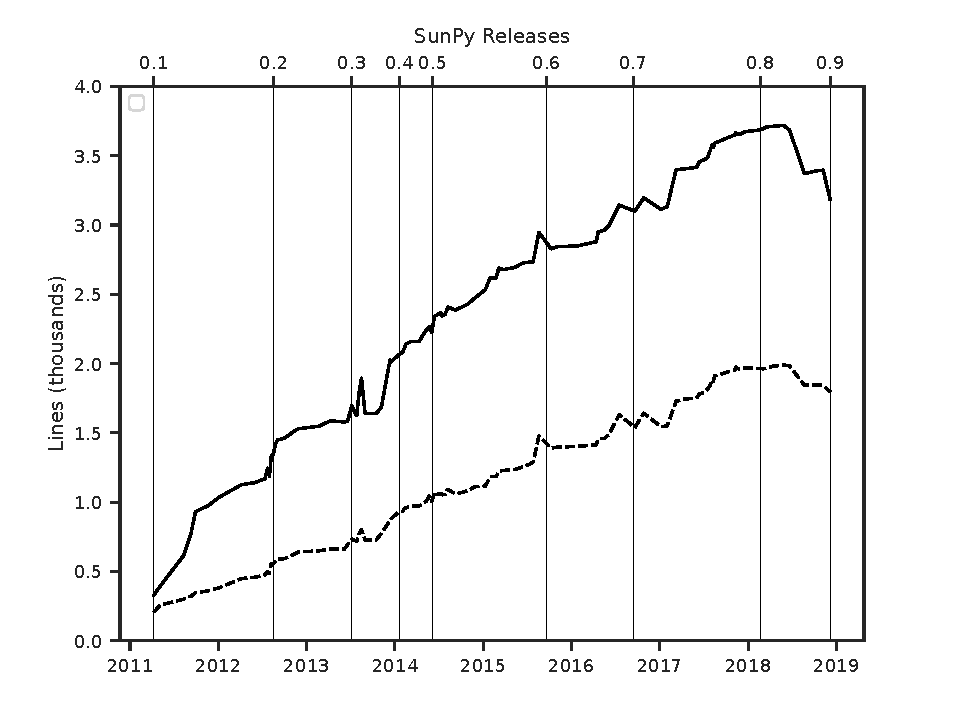
\includegraphics[width=0.5\textwidth]{figures/sunpy_history.pdf} &
  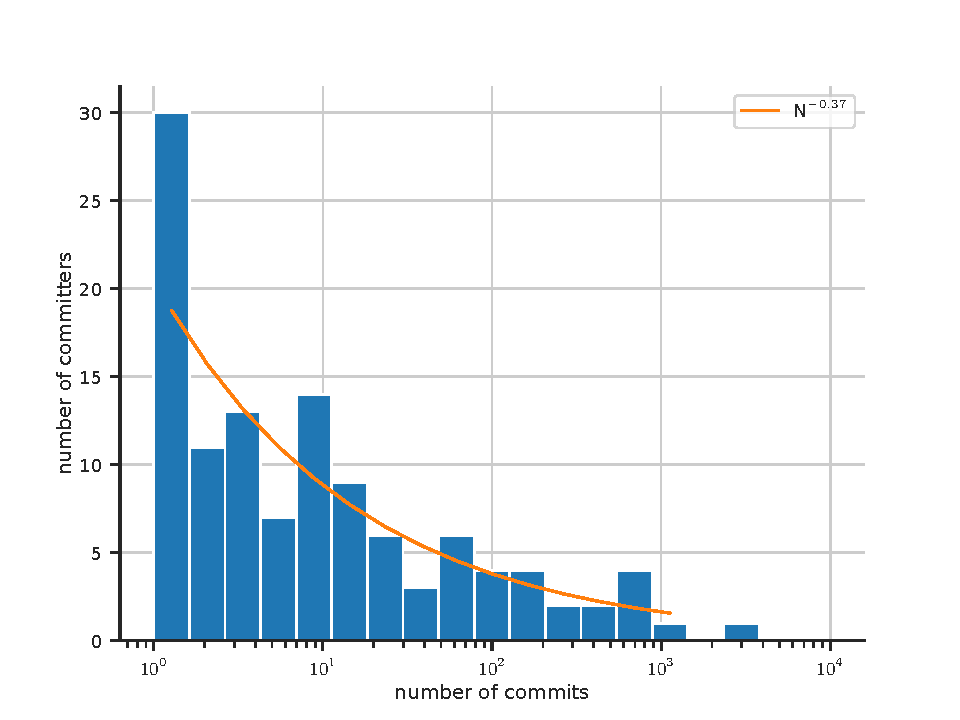
\includegraphics[width=0.5\textwidth]{figures/busfactor_plot.pdf} \\
(a) & (b)  \\
\end{tabular}
\begin{tabular}{c}
  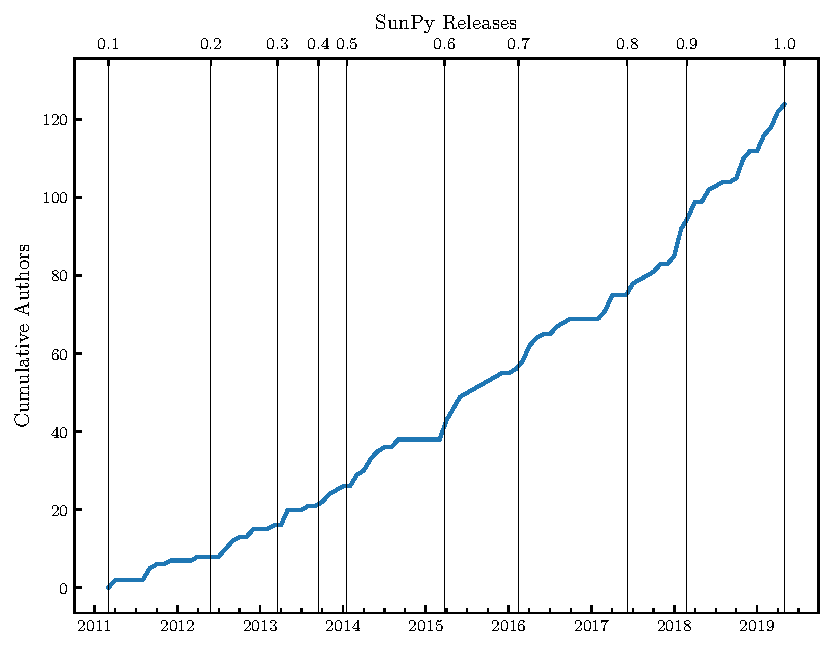
\includegraphics[width=0.5\textwidth]{figures/cumulative_authors.pdf} \\
(c)  \\
\end{tabular}
\caption{
	(a) This figure charts the amount of lines of Python code (dotted black line) and total line count (solid black line) with each major release of \sunpy.
	It details a steady increase of the \sunpypkg codebase with larger additions to our documentation over the last few major versions of \sunpypkg.
	The most striking are the reductions after version 0.9, going into 1.0.
	This was a period that undersaw major phases of code organization, deletion of obsolete features as well as removing Python 2 support.
	(b) This figure showcases the amount of authors to the number of commits they have done.
	It should be noted that the number of commits is not a 100\% useful measure as any one commit could have as many code or line changes as the previous 100 commits.
	However, it does indicate the majority of commits within the package are undertaken by the least amount of people with on average, contributions from an individual is typically less than 10 commits.
	(c) This figure charts the amount of authors (i.e., committers) to the \sunpypkg as a function of time.
	The package has seen a steady rise with time as word of mouth and the community around \sunpy has developed and grown.
	Two periods of time stand out, mid-2015 and early 2018, which saw a large increase in the amount of authors over a shorter period than normal.
}
\label{fig:image2}
\end{figure}
